\begin{figure}
    \centering    
{\footnotesize
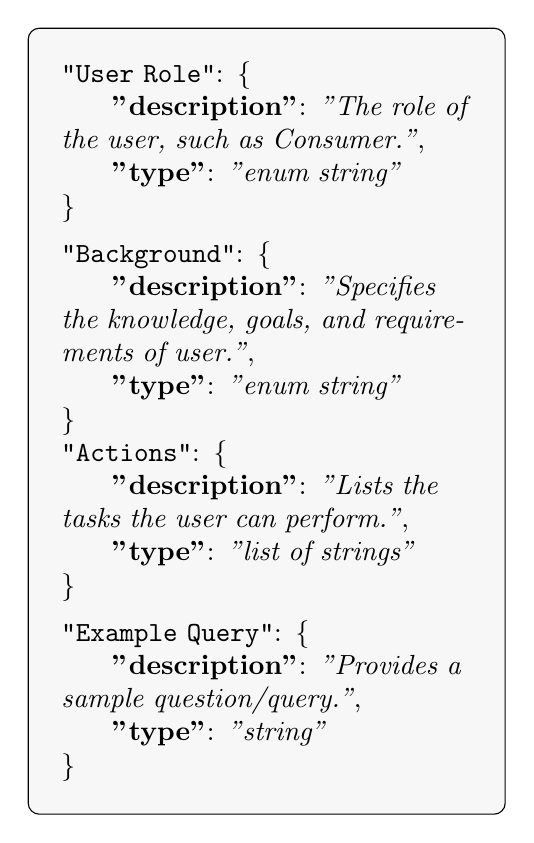
\begin{tikzpicture}
% Draw rounded rectangle with shadow
\node[rectangle, rounded corners, draw=black, fill=black!3!white, text width=0.43\textwidth, inner sep=12pt, align=left] (box) {
    \textbf{\texttt{"User Role"}}: \{\\
    \hspace{15pt} \textbf{"description"}: \textit{"The role of the user, such as Consumer."}, \\
    \hspace{15pt} \textbf{"type"}: \textit{"enum string"} \\
    \} \vspace{5pt}\\
    \textbf{\texttt{"Background"}}: \{\\
    \hspace{15pt} \textbf{"description"}: \textit{"Specifies the knowledge, goals, and requirements of user."}, \\
    \hspace{15pt} \textbf{"type"}: \textit{"enum string"} \\
    \} \\
    \textbf{\texttt{"Actions"}}: \{\\
    \hspace{15pt} \textbf{"description"}: \textit{"Lists the tasks the user can perform."}, \\
    \hspace{15pt} \textbf{"type"}: \textit{"list of strings"} \\
    \} \vspace{5pt}\\
    \textbf{\texttt{"Example Query"}}: \{\\
    \hspace{15pt} \textbf{"description"}: \textit{"Provides a sample question/query."}, \\
    \hspace{15pt} \textbf{"type"}: \textit{"string"} \\
    \}
};

\end{tikzpicture}
}
\caption{Use case specializations. For each use case, we define its role, goal, actions, and example query. For each property, we present its description and type.}
\label{fig:usecasedef}
\end{figure}